\NeedsTeXFormat{LaTeX2e}
\documentclass[11pt]{article}
\usepackage[utf8]{inputenc}

\usepackage{booktabs}
\usepackage{setspace}
\usepackage{amsmath}
\usepackage{amssymb}
\usepackage{epsfig}

\usepackage{marvosym}

\usepackage{graphicx}
\usepackage{caption}
\usepackage{subcaption}
\usepackage{multicol}
\usepackage{etoolbox}

\usepackage{tikz}

\def\checkmark{\tikz\fill[scale=0.4](0,.35) -- (.25,0) -- (1,.7) -- (.25,.15) -- cycle;} 

\setlength{\textheight}{9in}
\setlength{\textwidth}{6in}
\setlength{\oddsidemargin}{.25in}
\setlength{\topmargin}{-.5in} 

\patchcmd{\thebibliography}{\section*{\refname}}
    {\begin{multicols}{2}[\section*{\refname}\singlespace\footnotesize]}{}{}
\patchcmd{\endthebibliography}{\endlist}{\endlist\end{multicols}}{}{}

\hyphenation{itself}

\title{Results - Draft}
\author{Niklas Christoffer Petersen\\Trafikselskabet Movia} % \\ Possible thesis advisor:  I.\ M.\ Firstreader}

\begin{document}


\singlespace
\maketitle

\begin{abstract}                % ~350 words max
\end{abstract}

\onehalfspacing

% This sets section-numbering to only include Section and Subsection numbers
\setcounter{secnumdepth}{2}

\section{Background}\label{ch:background}

\section{Data}\label{ch:data}
\begin{table}[h!]
    \center
    \footnotesize
    \begin{tabular}{lrrrr}
\toprule
                                                  Link Name & Link Travel Time &      &    &     \\
                                                            &             Mean & Std. & p5 & p95 \\
\midrule
 Valby St. (10427) - Toftegårds Plads (1183) & 74 & 34 & 39 & 130 \\
 Toftegårds Plads (1183) - Vestre Kirkegård Nord (2673) & 67 & 22 & 45 & 98 \\
 Vestre Kirkegård Nord (2673) - Sankt Annæ Gymnasium (2675) & 66 & 24 & 54 & 87 \\
 Sankt Annæ Gymnasium (2675) - Sjælør St. (1188) & 52 & 14 & 41 & 78 \\
 Sjælør St. (1188) - Mozarts Plads (1190) & 88 & 20 & 62 & 122 \\
 Mozarts Plads (1190) - Bådehavnsgade (1192) & 154 & 48 & 93 & 228 \\
 Bådehavnsgade (1192) - Sluseholmen (1193) & 50 & 18 & 30 & 74 \\
\bottomrule
\end{tabular}

\end{table}

\begin{figure}[h!]
    \center
    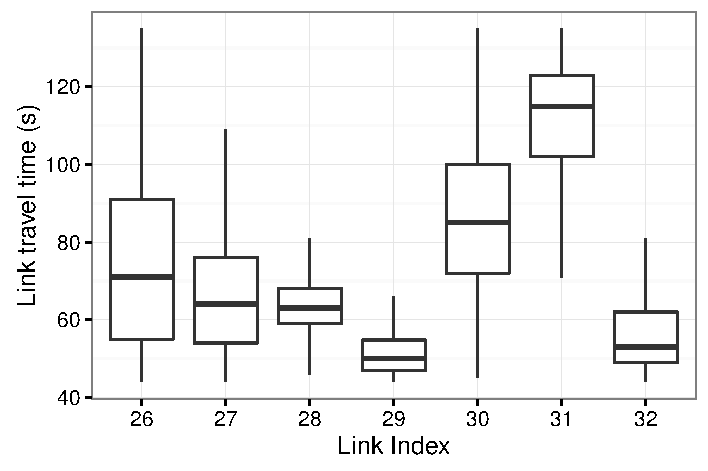
\includegraphics[scale=.8]{../plots/d1_loi_boxplot_nooutlier}
    \caption{}    
\end{figure}
\clearpage

\subsection{Outliers}
Slowest 5\% pr each link. Number of links in set for each journey.

\begin{figure}[h!]
    \center
    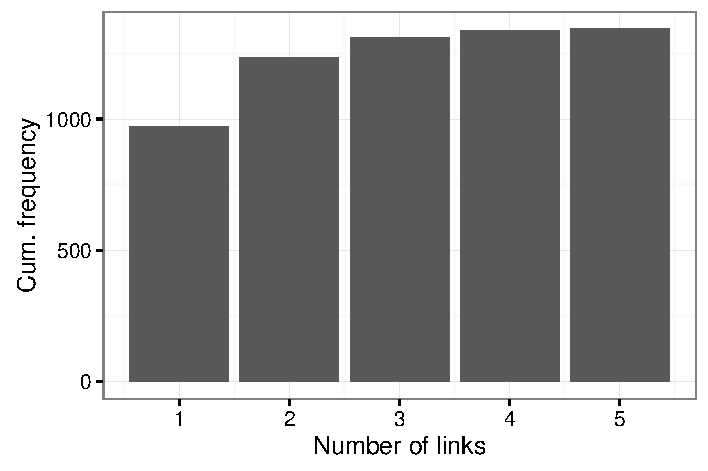
\includegraphics[scale=.8]{../plots/d1_loi_b5p_by_journeyref}
    \caption{}    
\end{figure}


\begin{figure}[h!]
    \center
    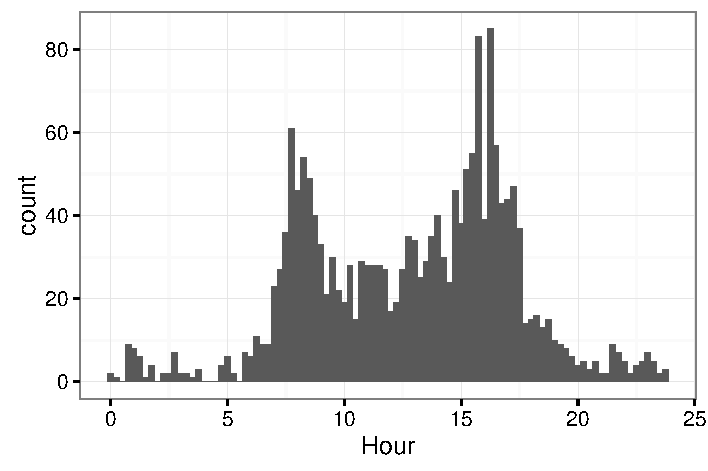
\includegraphics[scale=.8]{../plots/d1_loi_b5p_hour_histogram}
    \caption{}    
\end{figure}

\clearpage

\section{Results}\label{ch:results}

\subsection{General models}

\subsubsection{LR general models}

\begin{table}[!ht]
    \center
    \footnotesize
    \include{results_lr_single}
    \caption{Results using a single LR model.}
\end{table}

\subsubsection{SVR general models}

\begin{table}[!ht]
    \center
    \footnotesize
    \include{results_svr_single}
    \caption{Results using a single SVR model.}
\end{table}

\subsubsection{NN general models}

\begin{table}[!ht]
    \center
    \footnotesize
    \include{results_nn_single}
    \caption{Results using a single NN model.}
\end{table}



\subsection{Link models}

\subsubsection{LN link models}

\begin{table}[!ht]
    \center
    \footnotesize
    \include{results_lr_multiple}
    \caption{Results using multiple LR link models.}
\end{table}

\subsubsection{SVR link models}

\begin{table}[!ht]
    \center
    \footnotesize
    \include{results_svr_multiple}
    \caption{Results using multiple SVR link models.}
\end{table}

\subsubsection{NN link models}

\begin{table}[!ht]
    \center
    \footnotesize
    \include{results_nn_multiple}
    \caption{Results using a multiple NN model.}
\end{table}

\clearpage

\subsection{Single vs. multiple plots (SVR/NN)}

\begin{figure}[!ht]
    \center
    \includegraphics[width=\textwidth]{../plots/results_svr_errors.pdf}
    \caption{}    
\end{figure}

\begin{figure}[!ht]
    \center
    \includegraphics[width=\textwidth]{../plots/results_dnn_errors.pdf}
    \caption{}    
\end{figure}
\clearpage

\section{More inputs}
\begin{itemize}
    \item Peek non peek \checkmark
    \item no of Traffic ligths
    \item parking?
    \item roadworks
    \item weather
    \item proximity to station, stadion etc.
\end{itemize}

Future work:
- Distribution of error terms in single model vs. specialized models.
- Comapare models 
- Demand based models
- 


\begin{spacing}{1}
  \bibliographystyle{ieeetr}
  \bibliography{../references/library}
\end{spacing}

\end{document}
